\chapter{INTRODUCTION}
\label{introduction}
\section{Motivation}
Along with the development of technology, data is generated with a tremendous volume. According to the statistic, Facebook users upload 250 billion photos, and 350 million new images each day \footnote{Source: \url{https://www.businessinsider.com/facebook-350-million-photos-each-day-2013-9}}. In 2016, 47 \% of Vietnamese population have access to the Internet (World bank). This explosion of data enable the opportunity to analyze and extract valuable information.

One of the things that support the advancement of Deep Learning is the massive amount of data that is available today. This enables Neural Networks to really show their potential since they get better the more data you fed into them. Neural network is one of the most effective technique to derive information from data. In recent years, advancements in Neural Networks significantly enhanced the development of computer vision field. On the famous ImageNet \footnotetext{Source: \url:{http://www.image-net.org/challenges/LSVRC/}}dataset, trained neural networks can now generate results that are better than human in classifying images (Figure \ref{chap3:deeplearning_vs_human}). 

\begin{center}
    \begin{figure}[H]
    \centering
    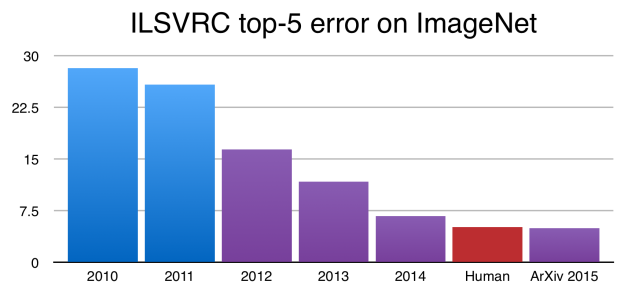
\includegraphics[width=0.75\columnwidth]{images/chap3/deeplearning_vs_human.png}
    \footcaption{Neural Network out-performing human in 2015 on ImageNet Large Scale Visual Recognition Challenge}
    \label{chap3:deeplearning_vs_human}
    \end{figure}
\end{center}
\footnotetext{Source: \url:{ https://devblogs.nvidia.com/mocha-jl-deep-learning-julia/}}
Availability of data and advancement of deep-learning poses a solution to strengthen the security: Collecting data and using deep learning to analyze collected data to improve security. 
In this modern and fast paced world, security is more important than ever. It is one of the fastest growing industries in the world today.
Almost everyday one hears about damage or loss occurring due to security lapses or a lack of security on the news. 

\section{Thesis statement}
\subsection{Goal}
Kha writes
The goal of this thesis is to accomplish to the following tasks:
\begin{itemize}
	\item Create an interface to interact with users. In the scope of this thesis, users of the system are inhabitants of a neighbor
	\item Create data collection points with proposing crowd-sourcing methods. Collected data can be in form of images and videos form contributors such as residents of neighbors, security camera.
	\item Analyze collected data using methods which will be proposed in the following chapters, and come up with meaningful information such as warnings or notifications to users of the system.
\end{itemize} 
Tri writes
The goal of this thesis is to build a system to collect and analyze image/video data using crowd-sourcing model and deep learning techniques for social security. The system require these features:
\begin{itemize}
	\item Using crowd-sourcing technique to collect image/video from users.
	\item Collected data are saved into a database.
	\item Extract valuable information from collected data using deep learning.
	\item Extracted information is also saved to database and used for security matter
\end{itemize} 
The main task of the project are:
\begin{itemize}
	\item Create an user interface to interact with users. The interface allows users to upload image/video and provide as much as information about the data to the system.
	\item Design a database which is able to save data, information about data, extracted information from data,...
	\item Design a deep learning model to extract information from data.
	\item Using extracted information to notify users about security problem.
\end{itemize} 

\subsection{Stages}
With specified tasks, the thesis is divided into 6 main stages:
\begin{itemize}
	\item Stage 1: Study and research crowd-sourcing methods, background theory of machine learning in general and deep learning in particular. Especially, research deep learning models appropriate to extract information from image/video
	\item Stage 2: Implement a module to handle image. 
	\item Stage 3: Design an applicable database.
	\item Stage 4: Implement a interface to interact with user.
	\item Stage 5: Implement a module to handle video
	\item Stage 6: Complete the system by connecting interface, image handling module, video handling module together. Output from image/video handling module is used to notify user about security problem through the interface.
\end{itemize} 
In proposal thesis, stage 1 and 2 of the project are done. Remaining stages are finished in thesis.  
\section{Scientific and Practical contributions}
\subsection{Scientific contributions}
Develop a system to collect data and allow user to interact with it through posting and notifications. \\
By applying Deep Learning and Computer Vision theories and by utilizing the Keras framework with a Tensorflow backend, some video classification techniques can be re-implemented and benchmarked. Subsequently, the team is able to apply those techniques to a real-world problem which is finding suspicious activities in videos \\ %FIX.
In addition, those classifying models are deployed with performance in mind using NGINX ,Gunicorn and Flask framework.
\subsection{Practical contributions}
The thesis proposes a system to improve security of neighborhoods. Such system can be beneficial to the residents as it assure their safety.
\section{Thesis scope}
Currently, building a system to enhance security for a whole city is impractical due to limited resources. The thesis focuses on building the system to raise security within a scope of a neighborhood. The scope can be freely expanded with additional resources in the future.
\section{Report overview}
\begin{itemize}
	\item Chapter 1: Introduce the main goal of the thesis, planned stages to conduct the project, overview of the report.
	\item Chapter 2: Background knowledge about ...
	\item Chapter 3: Propose a system consists of 2 subsystems: a social network website and an analysis system which contains a face recognition module and a video classifier module. 
	\item Chapter 4: The implementation of the social media website, face recognition module, video classifier module and connection between them.
	\item Chapter 5: 
	\item Chapter 6: Result, limitation and how to resolve these challenges, further development in the future.
	\item Chapter 7: References
\end{itemize} 
